\documentclass[12pt,a4paper]{report}

\usepackage[czech]{babel}
\usepackage[utf8]{inputenc}
\usepackage[T1]{fontenc}
\usepackage{hyperref}
\usepackage{graphicx}
\usepackage{geometry}
\usepackage{biblatex}
\usepackage{subcaption} % Pro použití subfigure prostředí

\addbibresource{bib.bib}

\geometry{a4paper, margin=2.5cm}

% Titulní strana
\title{Mobilní aplikace pro inzerci a adopci domácích zvířat}
\author{Adam Míka}
\date{31. prosince 2024}

\begin{document}

\maketitle

\chapter*{Abstrakt}
Text abstraktu v jazyce práce, tj. zde česky.

\chapter*{Abstract}
The abstract text in a secondary language, here in English.

\chapter*{Poděkování}
Text poděkování.

\tableofcontents

\chapter{Úvod}
V současné době moderních technologií hrají mobilní aplikace klíčovou roli v mnoha aspektech každodenního života. Jednou z oblastí, kde mohou tyto technologie přinést výrazný přínos, je péče o domácí zvířata. Téma adopce a inzerce domácích zvířat je stále aktuálnější, přičemž potřeba inovativních řešení je více než zřejmá. Rostoucí počet opuštěných zvířat v útulcích a zájem o odpovědné vlastnictví zvířat vyžadují efektivní nástroje pro propojení zájemců o adopci s majiteli zvířat.

Cílem této práce je návrh a realizace mobilní aplikace, která bude sloužit jako moderní a uživatelsky přívětivá platforma pro inzerci a adopci domácích zvířat. Vytvořená aplikace bude uživatelům umožňovat snadné prohlížení inzerátů a filtrování podle specifických kritérií (například druhu zvířat, lokace nebo věku). Kromě toho nabídne intuitivní uživatelské rozhraní, které bude snadno ovladatelné i pro méně technicky zdatné uživatele.

Analýza stávajících řešení ukazuje, že dostupné aplikace často nevyhovují požadavkům moderních uživatelů. Mnoho z nich postrádá klíčové funkce nebo je orientováno pouze na webové prostředí. Tyto nedostatky ztěžují proces adopce a snižují efektivitu stávajících platforem. Navržená aplikace se zaměří na odstranění těchto nedostatků a nabídne komplexní řešení, které bude reflektovat potřeby cílové skupiny.

Motivací pro tuto práci je nejen zlepšení procesu adopce zvířat, ale také zvýšení povědomí o odpovědném vlastnictví domácích zvířat. Mobilní aplikace jako centralizovaný nástroj umožní propojení uživatelů s databázemi útulků, zjednoduší správu inzerátů a podpoří snahu o nalezení vhodného domova pro zvířata v nouzi. Výsledkem práce bude funkční aplikace, jejíž struktura a možnosti budou navrženy s ohledem na další rozšíření, jako je například integrace s veterinárními službami nebo sociálními sítěmi.

Tato práce si klade za cíl nejen vyvinout funkční produkt, ale také přispět k řešení společenského problému a ukázat, jak lze moderní technologie využít pro podporu dobré věci.


\chapter{Analýza existujících řešení}

Tato kapitola je zaměřena na analýzu dostupných softwarových řešení, která se specializují na inzerci a adopci domácích zvířat. Cílem této analýzy je prozkoumat funkce, uživatelské rozhraní a přístupy jednotlivých aplikací, identifikovat jejich výhody a nevýhody a na základě získaných poznatků formulovat doporučení pro návrh nové aplikace.

Analýza zahrnuje webové i mobilní aplikace, které slouží k podobným účelům, jako je zamýšlený projekt. Pro hodnocení aplikací byly zvoleny následující kritéria:
\begin{itemize}
    \item Rozsah a kvalita nabízených funkcí (např. vyhledávání zvířat, proces adopce, registrace útulků).
    \item Uživatelská přívětivost a intuitivnost rozhraní.
    \item Celkový přínos pro cílovou skupinu uživatelů.
    \item Technologická řešení a možnosti rozšiřitelnosti aplikace.
\end{itemize}

Následující sekce detailně rozebírají jednotlivé vybrané aplikace. Hodnocení se zaměřuje na klíčové aspekty, jako je funkčnost a uživatelský zážitek, a následně je doplněno shrnutím hlavních zjištění.

\section{Přehled dostupných softwarových řešení}

V oblasti adopcí a inzercí domácích zvířat existuje řada softwarových řešení, která se liší svou zaměřeností, funkcionalitou a cílovou skupinou uživatelů. Tato řešení lze rozdělit do kategorií zahrnujících webové portály a mobilní aplikace. Následující přehled shrnuje klíčové vlastnosti vybraných softwarových řešení.

\subsection{Webové portály}

V následující části jsou popsány webové portály, které hrají významnou roli v oblasti adopce a inzerce domácích zvířat. Jedná se o české i zahraniční platformy zaměřené na propojení útulků se zájemci o adopci, přičemž každá z nich nabízí specifické funkce a přístupy.

\begin{itemize}
    \item \textbf{Pesweb} – Tento český portál se zaměřuje na inzerci psů a koček k adopci. Umožňuje uživatelům vyhledávat zvířata podle specifických parametrů, jako je věk, velikost nebo plemeno. Důležitou funkcí je také možnost přímého kontaktu s útulky prostřednictvím platformy. Mezi hlavní výhody patří přehlednost a jednoduchost uživatelského rozhraní.

    \item \textbf{Voriskov} –- Online útulek rozšiřující nabídku i na další druhy domácích mazlíčků, jako jsou hlodavci nebo ptáci. Portál nabízí uživatelsky přívětivé prostředí, ale jeho nabídka se primárně zaměřuje na psy. Jedná se o jednoduchý a intuitivní systém vhodný pro široké spektrum uživatelů.

    \item \textbf{Dog-point} –- Webový portál specializovaný výhradně na adopci psů. Nabízí podrobné profily zvířat, které zahrnují informace o jejich zdravotním stavu, povahových rysech a základních požadavcích na péči. Portál se zaměřuje na přehlednou prezentaci informací a efektivní propojení zájemců s útulkem.

    \item \textbf{Puppio} –- Český webový portál zaměřený na inzerci domácích mazlíčků. Portál se specializuje výhradně na inzerce zvířat ze Středočeského kraje. Jedná se o regionálně orientovanou platformu, která klade důraz na jednoduché uživatelské prostředí a základní vyhledávací funkce.

    \item \textbf{Anidef} – Online webový útulek zaměřený na adopce nejen psů a koček, ale i dalších druhů zvířat, jako jsou kozy, krávy, králíci nebo holubi. Platforma poskytuje základní informace o zvířatech nabízených k adopci, včetně věku, plemene a aktuálního zdravotního stavu. Portál neobsahuje pokročilé funkce ani integrovaný systém pro správu adopcí, jeho hlavním cílem je však rozšíření možností adopce na širší spektrum zvířat.
\end{itemize}

Webové portály popsané výše představují důležitou součást ekosystému adopce domácích zvířat. Každý z nich je charakteristický svým zaměřením a přístupem k řešení potřeb uživatelů. Přestože nabízejí širokou škálu funkcí, identifikovány byly i určité mezery, které budou dále rozebrány v detailní analýze.


\subsection{Mobilní aplikace}
\begin{itemize}
    \item \textbf{Petfinder} – Mobilní aplikace, která propojuje zájemce o adopci s útulky v Severní Americe. Nabízí pokročilé vyhledávací funkce a personalizovaná doporučení, avšak její dostupnost je geograficky omezená pouze na tento region.
\end{itemize}

Tento přehled poskytuje základní orientaci v dostupných řešeních. Zároveň ukazuje, že stávající nabídka aplikací a portálů je často omezena na specifické funkce nebo geografická území, což otevírá prostor pro inovativní a komplexnější přístup k problematice adopce domácích zvířat. V následujících částech se budeme věnovat detailní analýze těchto řešení.

\section{Detailní analýza vybraných aplikací}

Tato část práce se podrobně zabývá analýzou jednotlivých aplikací zaměřených na adopci domácích zvířat. Výběr zahrnuje jak české aplikace, například \textbf{Pesweb} nebo \textbf{Anidef}, tak zahraniční platformy jako \textbf{Petfinder}. Cílem této analýzy je zhodnotit jejich funkce, uživatelské rozhraní a celkový přínos pro uživatele.

Každá aplikace bude stručně představena, následně budou uvedeny její hlavní výhody a nevýhody. Součástí analýzy budou i vizuální ukázky aplikací ve formě přiložených snímků obrazovek nebo uživatelských rozhraní. Tyto ukázky napomohou ilustrovat klíčové aspekty, jako je přehlednost a intuitivnost designu. \\

\noindent Hodnocení bude rozděleno do následujících kategorií:\\

\noindent\textbf{Funkčnost}: Nabízené funkce, jejich rozsah a přizpůsobení potřebám uživatelů.\\

\noindent\textbf{Uživatelské rozhraní}: Přehlednost, jednoduchost a estetika designu.\\

\noindent\textbf{Technologická řešení}: Použité technologie, možnosti integrace a rozšiřitelnost.\\

\noindent\textbf{Regionální dostupnost}: Geografická omezení a přístupnost pro uživatele.\\

\subsection{Pesweb}

\noindent \textbf{Funkčnost}: Portál nabízí možnost vyhledávání zvířat podle různých parametrů, jako jsou věk, velikost či plemeno, a umožňuje přímou komunikaci s útulky. Přesto postrádá pokročilé funkce, jako je personalizace vyhledávání na základě uživatelských preferencí nebo automatizace adopčního procesu, což omezuje jeho komplexnost.\\

\noindent \textbf{Uživatelské rozhraní}: Uživatelské rozhraní je navrženo jednoduše a intuitivně, což usnadňuje jeho využívání i méně technicky zdatným uživatelům. Některé grafické prvky by však mohly být upraveny tak, aby lépe odpovídaly požadavkům uživatelů na moderní vizuální přehlednost a estetiku. Navíc chybějící optimalizace pro mobilní zařízení může uživatelům s menšími obrazovkami způsobovat komplikace při navigaci po portálu.\\

\noindent\textbf{Technologická řešení}: Portál funguje pouze ve webovém prostředí a nenabízí podporu mobilních aplikací. Výkon systému je pomalý, zejména při přepínání mezi sekcemi, což může negativně ovlivnit uživatelský zážitek.\\

\noindent \textbf{Regionální dostupnost}: Platforma je zaměřena výhradně na Českou republiku, přičemž poskytuje pokrytí po celé zemi. Tento přístup podporuje dostupnost zvířat z regionálních útulků pro zájemce o adopci.\\

\begin{figure}[h!]
    \centering
    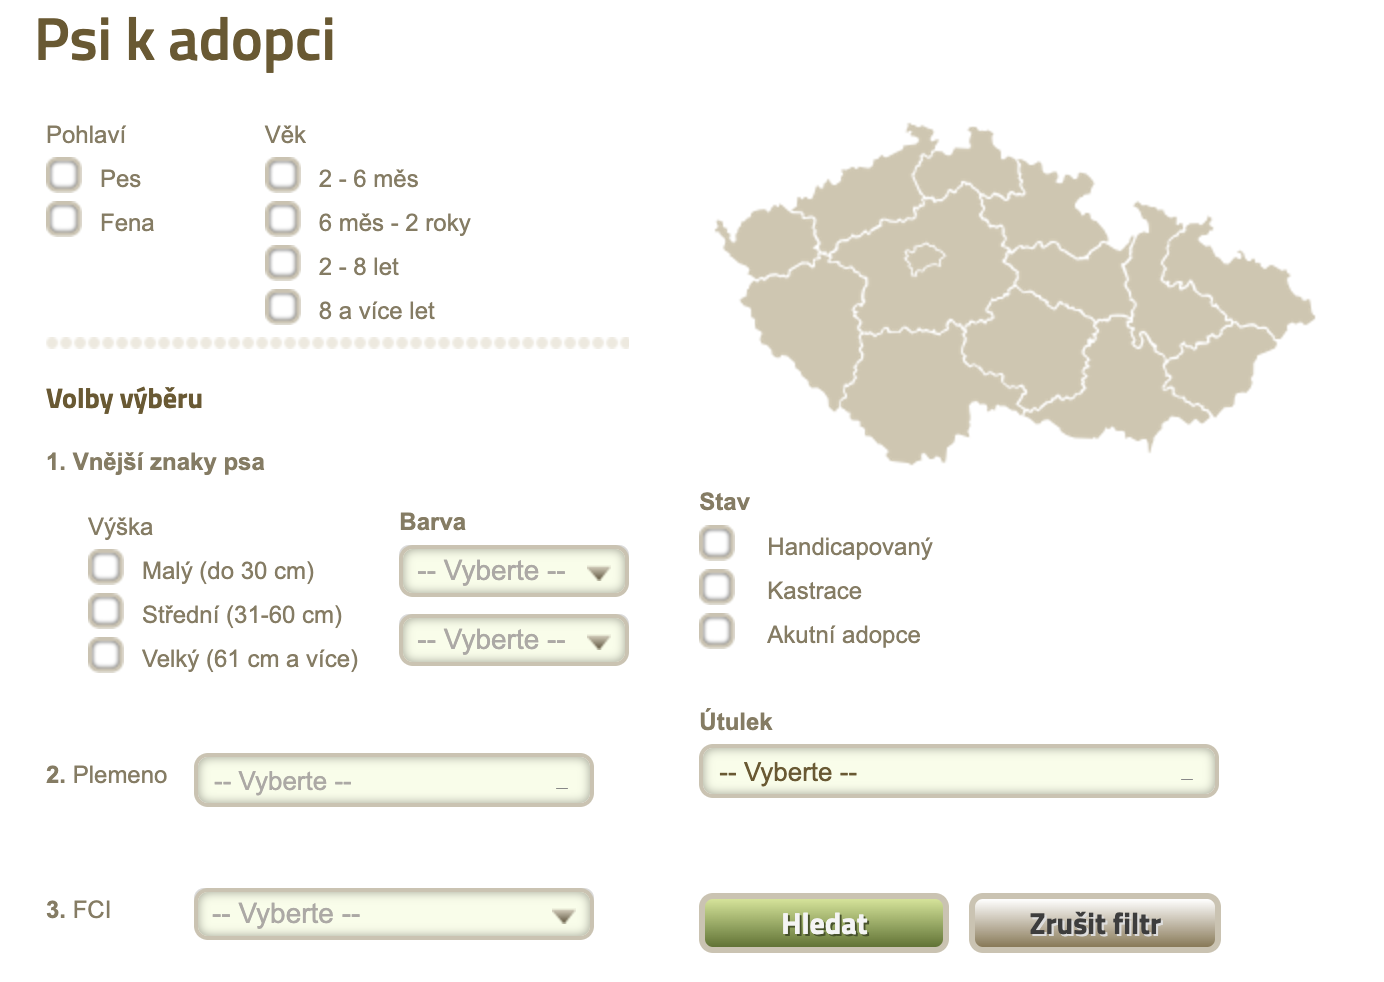
\includegraphics[width=0.8\textwidth]{img/pesweb.png} % Cesta k obrázku
    \caption{Filtrace záznamů na portále Pesweb} % Popis obrázku
    \label{fig:pesweb_filter} % Identifikátor pro odkazování na obrázky
\end{figure}

\pagebreak

\subsection{Anidef}

\noindent \textbf{Funkčnost}: Platforma poskytuje základní informace o zvířatech, včetně věku, plemene a zdravotního stavu. Nicméně postrádá pokročilé adopční funkce, jako je personalizace na základě preferencí uživatele, možnost sledování adopcí nebo filtrování podle kritérií, jako jsou plemeno, velikost či věk, což omezuje její praktičnost.\\

\noindent\textbf{Uživatelské rozhraní}: Rozhraní je jednoduché a uživatelsky přívětivé, což zajišťuje snadnou orientaci pro většinu uživatelů. Některé aspekty grafického návrhu by však mohly být upraveny tak, aby lépe odpovídaly očekáváním uživatelů preferujících vizuálně propracovanější aplikace, což by mohlo zvýšit jeho atraktivitu pro mladší uživatele.\\

\noindent\textbf{Technologická řešení}: Platforma je dostupná výhradně jako webový portál, což omezuje její využití na mobilních zařízeních, jelikož chybí nativní mobilní aplikace nebo integrace s dalšími systémy. Proces adopce je realizován prostřednictvím Google formuláře, jehož délka a struktura mohou být pro některé zájemce méně přívětivé.\\
 
\noindent \textbf{Regionální dostupnost}: Služby jsou geograficky omezeny na Českou republiku a vztahují se pouze k určitému konkrétnímu útulku, což snižuje jejich flexibilitu pro uživatele z jiných regionů.\\

\subsection{Petfinder}

\noindent \textbf{Funkčnost}: Aplikace nabízí pokročilé vyhledávací funkce, včetně možnosti filtrování zvířat podle druhu, věku nebo lokality. Kromě toho obsahuje personalizovaná doporučení na základě uživatelských preferencí, což zlepšuje uživatelský zážitek.\\

\noindent \textbf{Uživatelské rozhraní}: Uživatelské rozhraní je jednoduché a funkční, avšak některé designové prvky by mohly být optimalizovány, aby lépe odpovídaly očekáváním uživatelů v oblasti pohodlného a plynulého ovládání. Určité nedostatky mohou snižovat celkový uživatelský zážitek, zejména při použití na mobilních zařízeních.\\

\noindent \textbf{Technologická řešení}: Aplikace využívá geolokaci a algoritmy pro personalizaci doporučení, což ji činí technologicky vyspělou. Její využití je však omezeno na Severní Ameriku, což značně snižuje dostupnost pro uživatele z jiných regionů.\\

\noindent \textbf{Regionální dostupnost}: Aplikace je geograficky dostupná výhradně pro uživatele v Severní Americe, což omezuje její globální využití a atraktivitu pro širší publikum.\\

\begin{figure}[h!]
    \centering
    % První obrázek vlevo
    \begin{subfigure}{0.22\textwidth}
        \centering
        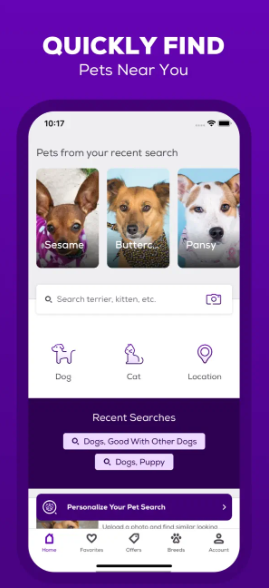
\includegraphics[width=\textwidth]{img/petfinder1.png} % Nahraďte správnou cestou
        \caption{Hlavní stránka} % Popis prvního obrázku
        \label{fig:obrazek1}
    \end{subfigure}
    \hfill
    % Druhý obrázek vpravo
    \begin{subfigure}{0.22\textwidth}
        \centering
        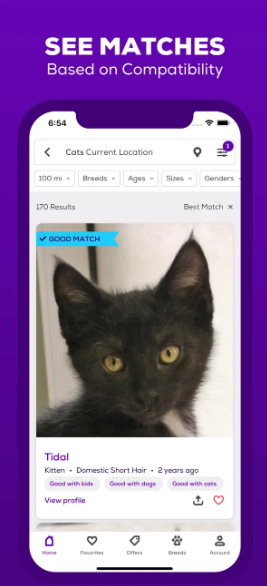
\includegraphics[width=\textwidth]{img/petfinder2.png} % Nahraďte správnou cestou
        \caption{Vybrané zvířata} % Popis druhého obrázku
        \label{fig:obrazek2}
    \end{subfigure}
    \hfill
    % Druhý obrázek vpravo
    \begin{subfigure}{0.22\textwidth}
        \centering
        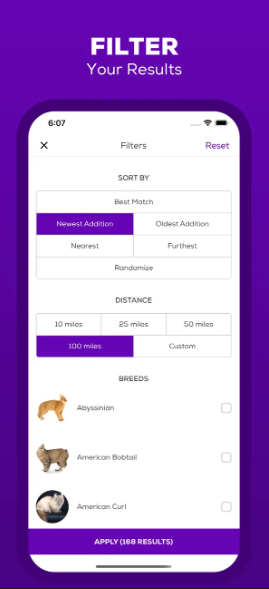
\includegraphics[width=\textwidth]{img/petfinder3.png} % Nahraďte správnou cestou
        \caption{Filtrace} % Popis druhého obrázku
        \label{fig:obrazek3}
    \end{subfigure}
    \hfill
    % Druhý obrázek vpravo
    \begin{subfigure}{0.22\textwidth}
        \centering
        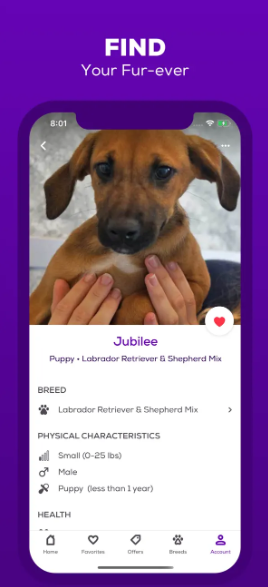
\includegraphics[width=\textwidth]{img/petfinder4.png} % Nahraďte správnou cestou
        \caption{Detail zvířete} % Popis druhého obrázku
        \label{fig:obrazek4}
    \end{subfigure}
    
    % Popisek pod celou skupinou obrázků
    \caption{Ukázky uživatelského rozhraní aplikace Petfinder} % Celkový popis
    \label{fig:obrazky-vedle-sebe}
\end{figure}


\subsection{Dog-point}

\noindent \textbf{Funkčnost}: Portál se zaměřuje na adopci psů, přičemž nabízí i možnost virtuální adopce pro psy s postižením, kteří nemohou být adoptováni. Kromě toho si zde uživatelé mohou zakoupit ručně vyráběné náramky, přívěsky a pamlsky pro své mazlíčky. Další poskytované služby zahrnují venčení, výcvik a odchyt psů. Hlavní nevýhodou je umístění útulku mimo dosah velkých měst, což může komplikovat dostupnost pro některé uživatele. Portál se specializuje výhradně na psy, což omezuje širší nabídku pro jiná domácí zvířata.\\

\noindent \textbf{Uživatelské rozhraní}: Design je přehledný a umožňuje snadnou orientaci, avšak proces adopce není plně intuitivní. Vyžaduje stažení dokumentů a jejich ruční vyplňování, což může být pro některé uživatele časově náročné a nekomfortní. Chybějící plně automatizovaný online proces snižuje celkovou uživatelskou přívětivost.\\

\noindent \textbf{Technologická řešení}: Portál funguje jako responzivní webová aplikace, která však nenabízí podporu pro nativní mobilní aplikace ani možnost integrace s jinými platformami.\\

\noindent \textbf{Regionální dostupnost}: Portál je dostupný pouze pro uživatele v České republice. Samotné umístění útulku znevýhodňuje uživatele z odlehlejších regionů, jako je například Plzeňský kraj.\\


\subsection{Puppio}

\noindent \textbf{Funkčnost}: Webový portál zaměřený na inzerci psů a koček z různých útulků. Nabízí možnost vyhledávání zvířat podle různých kritérií, jako je věk, plemeno nebo lokalita. Mezi hlavní výhody patří jednoduchost a přehlednost uživatelského rozhraní, které usnadňuje orientaci a vyhledávání zvířat. Nevýhodou je však zaměření pouze na Středočeský kraj a podle aktivity na sociálních sítích se zdá, že portál není delší dobu aktivní.\\

\noindent \textbf{Uživatelské rozhraní}: Jednoduché a přehledné rozhraní, vhodné pro základní inzerci. Portál nabízí přehledně zpracované informace o zvířatech, což může být inspirací pro návrh vlastní aplikace.\\

\noindent \textbf{Technologická řešení}: Omezeno na webové prostředí, bez podpory mobilních aplikací nebo možnosti integrace s dalšími systémy.\\

\noindent \textbf{Regionální dostupnost}: Zaměřuje se výhradně na inzeráty z oblasti Středočeského kraje.\\

\begin{figure}[h!]
    \centering
    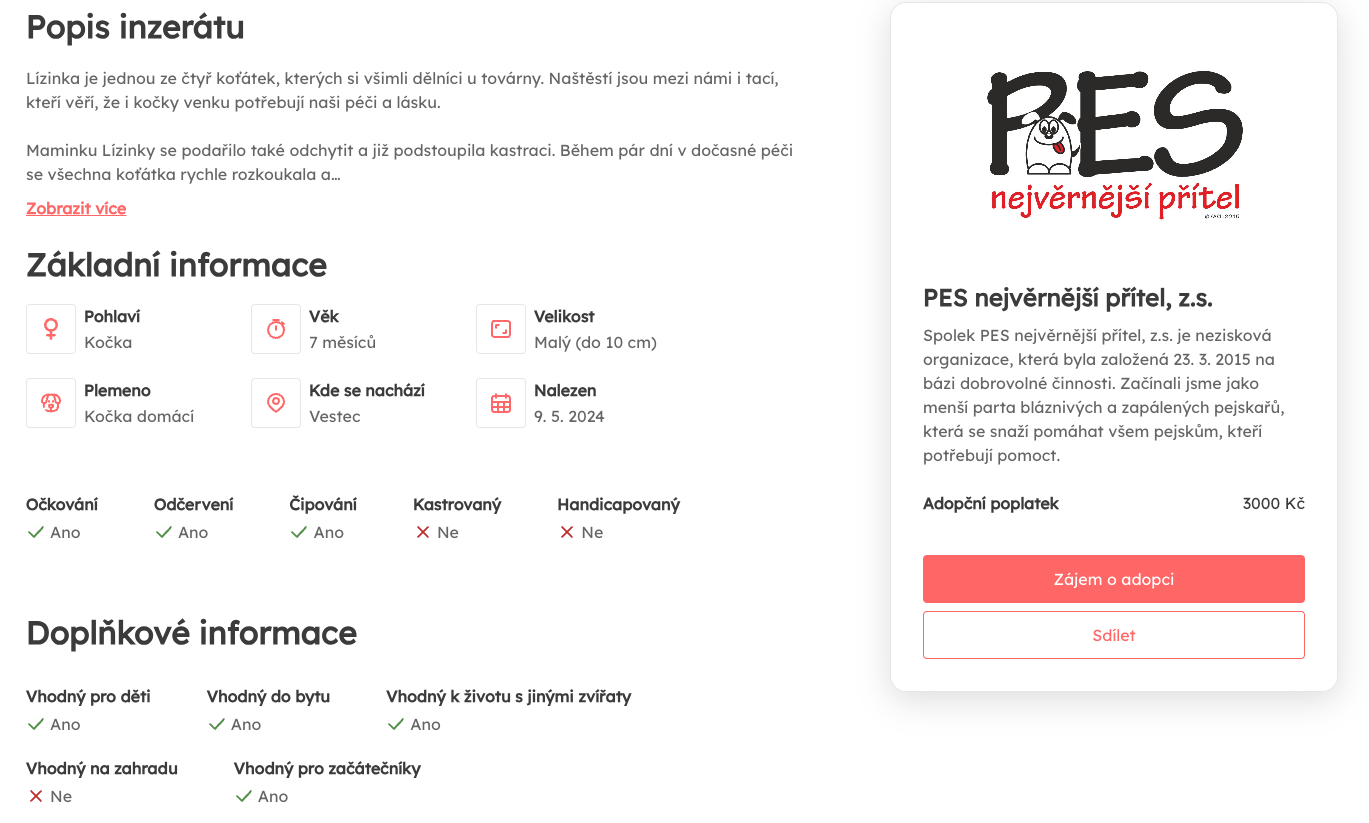
\includegraphics[width=0.8\textwidth]{img/puppio.png} % Cesta k obrázku
    \caption{Základní informace o zvířeti na portálu Puppio} % Popis obrázku
    \label{fig:basic-info-puppio} % Identifikátor pro odkazování na obrázky
\end{figure}

\pagebreak

\section{Srovnání dostupných řešení}

\begin{table}[h!]
    \centering
    \begin{tabular}{|l|c|c|c|c|c|}
        \hline
        \textbf{Srovnání} & \textbf{Pesweb} & \textbf{Anidef} & \textbf{Petfinder} & \textbf{Dog-point} & \textbf{Puppio} \\ \hline
        Filtrace zvířat & Ano & Ne & Ano & Ne & Ano \\ \hline
        Široká nabídka & Omezený & Ano & Ano & Ne & Omezený \\ \hline
        Podpora mobilních zařízení & Ne & Omezený & Ano & Omezený & Omezený \\ \hline
        Regionální dostupnost & Neomezený & Omezený & Omezený & Omezený & Omezený \\ \hline
    \end{tabular}
    \caption{Srovnání dostupných řešení pro adopci a inzerci zvířat}
    \label{tab:srovnani-reseni}
\end{table}

\subsection{Shrnutí zjištění}

Tabulka \ref{tab:srovnani-reseni} nabízí přehled hlavních charakteristik analyzovaných platforem:\\

\noindent \textbf{Filtrace zvířat}: Možnost filtrace zvířat je dostupná na platformách Pesweb, Petfinder a Puppio. Z těchto řešení vyniká Petfinder, který nabízí pokročilé možnosti filtrace.\\

\noindent \textbf{Široká nabídka}: Širokou nabídku zvířat poskytují platformy Petfinder a Anidef. Ostatní platformy mají omezený nebo úzce zaměřený obsah.\\

\noindent \textbf{Podpora mobilních zařízení}: Plnou podporu mobilních zařízení nabízí pouze Petfinder. Platformy Anidef, Dog-point a Puppio mají alespoň částečnou podporu ve formě responzivního designu. Pesweb naopak mobilní zařízení nepodporuje vůbec.\\

\noindent \textbf{Regionální dostupnost}: Platforma Pesweb nabízí nejširší geografické pokrytí s dostupností po celé České republice. Naopak ostatní platformy, včetně Dog-point a Puppio, jsou geograficky omezené na specifické regiony. Petfinder je omezen na Severní Ameriku.\\

Tato analýza ukazuje, že Petfinder má pokročilé funkce a mobilní podporu, ale jeho regionální omezení značně snižuje jeho dostupnost. Pesweb má široké pokrytí a základní funkce, ale zaostává v podpoře moderních technologií. Anidef a Puppio se zaměřují na specifické regiony, přičemž Puppio nabízí moderní design, ale chybí mu širší funkcionalita.\\


\chapter{Návrh nového řešení}

Na základě provedené analýzy stávajících softwarových řešení byla identifikována řada nedostatků, které nová aplikace plánuje odstranit. Tato kapitola se zaměřuje na návrh aplikace pro inzerci a adopci domácích zvířat, přičemž cílem je vytvořit moderní, uživatelsky přívětivou a funkčně bohatou mobilní aplikaci.

\section{Sběr požadavků}

Z provedené analýzy a hodnocení uživatelských očekávání vyplývají následující požadavky na novou aplikaci:\\

\noindent \textbf{Pokročilé filtrování zvířat}: Možnost filtrování podle druhu, věku, velikosti, lokality a dalších kritérií.\\

\noindent \textbf{Uživatelská personalizace}: Doporučení zvířat na základě preferencí uživatele.\\

\noindent \textbf{Optimalizace pro mobilní zařízení}: Plně responzivní aplikace dostupná pro Android a iOS.\\

\noindent \textbf{Datová integrace s útulky}: Správa informací o zvířatech v reálném čase.\\

\noindent \textbf{Jednoduchá registrace a správa profilu}: Pro zájemce o adopci a útulky.\\

\section{Uživatelské persony a případy užití}

Aby aplikace vyhovovala potřebám cílové skupiny, byly vytvořeny uživatelské persony a scénáře použití, které reflektují nejčastější interakce uživatelů s aplikací.
\pagebreak
\subsection{Zájemce o adopci}
\begin{table}[h!]
    \centering
    \renewcommand{\arraystretch}{1.4}
    \begin{tabular}{|p{3cm}|p{10cm}|}
        \hline
        \textbf{Popis} & Uživatel hledající vhodné zvíře k adopci. \\ \hline
        \textbf{Cíl} & Najít zvíře dle preferencí, prohlédnout informace a dokončit adopční proces. \\ \hline
        \textbf{Scénář použití} &
        \begin{itemize}
            \item Registrace do aplikace a vyplnění profilu.
            \item Použije filtry (věk, plemeno, lokalita) k vyhledání zvířat.
            \item Prohlédne si detailní informace o vybraném zvířeti.
            \item Kontaktuje útulek s žádostí o adopci.
        \end{itemize} \\ \hline
    \end{tabular}
    \caption{Persona: Zájemce o adopci.}
    \label{tab:persona_adopter}
\end{table}

\subsection{Zaměstnanec útulku}
\begin{table}[h!]
    \centering
    \renewcommand{\arraystretch}{1.4}
    \begin{tabular}{|p{3cm}|p{10cm}|}
        \hline
        \textbf{Popis} & Pracovník útulku spravující nabídku zvířat k adopci. \\ \hline
        \textbf{Cíl} & Přidat nová zvířata do systému a sledovat stav adopčních žádostí. \\ \hline
        \textbf{Scénář použití} &
        \begin{itemize}
            \item Registruje útulek do aplikace a nahraje nové zvíře s fotografiemi a podrobnými informacemi.
            \item Sleduje adopční žádosti a komunikuje mimo aplikaci s uživateli.
        \end{itemize} \\ \hline
    \end{tabular}
    \caption{Persona: Zaměstnanec útulku.}
    \label{tab:persona_shelter_worker}
\end{table}


\section{Návrh aplikace}

\subsection{Hlavní obrazovka aplikace}

Hlavní obrazovka aplikace slouží jako výchozí bod pro uživatele a poskytuje přehledné rozhraní pro navigaci a interakci s klíčovými funkcemi aplikace. Její návrh se zaměřuje na intuitivní ovládání a rychlý přístup k potřebným informacím.\\

\noindent \textbf{Spodní navigační panel}: Obsahuje ikony pro rychlý přístup k hlavním sekcím aplikace, jako jsou \textit{Domů}, \textit{Vyhledávání}, \textit{Oblíbené} a \textit{Profil}. Navigace je umístěna ve spodní části obrazovky pro snadnou dostupnost při ovládání jednou rukou.\\

\noindent \textbf{Vyhledávací panel}: Nachází se v horní části obrazovky a umožňuje vyhledávání zvířat podle různých kritérií. Mezi dostupné filtry patří:
\begin{itemize}
    \item Druh zvířete (pes, kočka, jiná zvířata),
    \item Věk,
    \item Plemeno,
    \item Lokalita.
\end{itemize}

\noindent \textbf{Výsledky vyhledávání}: Zobrazeny ve formě přehledných karet, které obsahují:

\begin{itemize}
    \item Fotografie zvířete,
    \item Základní informace (jméno, druh, věk, lokalita).
\end{itemize}

Kliknutím na kartu se uživateli zobrazí detailní informace o zvířeti, včetně dalších fotografií, podrobného popisu a možnosti kontaktovat útulek.\\

\noindent \textbf{Zájem o adopci}: Uživatel může vyjádřit zájem o zvíře stisknutím tlačítka s ikonou srdce nebo přetažením karty doprava.\\

\noindent \textbf{Odmítnutí zvířete}: Přetažením karty doleva může uživatel zvíře odmítnout a pokračovat ve vyhledávání.\\

\noindent \textbf{Kontaktování útulku}: V případě výrazného zájmu má uživatel možnost stisknout tlačítko s ikonou vlaštovky a přímo kontaktovat útulek.\\

\begin{figure}[h!]
    \centering
    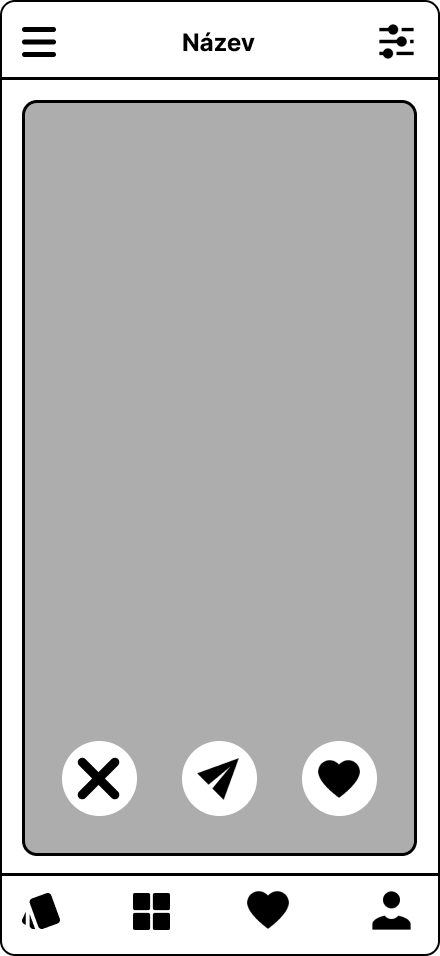
\includegraphics[width=0.25\textwidth]{img/Main.png}
    \caption{Návrh hlavní obrazovky aplikace.}
    \label{fig:home_screen}
\end{figure}

Hlavní obrazovka aplikace je navržena s důrazem na jednoduchost, přehlednost a efektivní ovládání, aby co nejvíce usnadnila uživatelům proces vyhledávání a adopce zvířat.

\newpage

\subsection{Vyhledávací obrazovka}

Vyhledávací obrazovka je navržena tak, aby uživatelům umožnila efektivní procházení nabídky zvířat a aplikaci přizpůsobila jejich konkrétním požadavkům. Tato obrazovka poskytuje širší možnosti vyhledávání oproti hlavní obrazovce a přináší intuitivní přístup k jednotlivým kategoriím.\\

\noindent \textbf{Spodní navigační panel}: Stejně jako na hlavní obrazovce, i zde je k dispozici navigační panel ve spodní části obrazovky, který umožňuje rychlý přístup k sekcím aplikace.\\

\noindent \textbf{Hlavní dlaždice}: Vyhledávací rozhraní obsahuje tři základní dlaždice pro rychlou navigaci:
\begin{itemize}
    \item \textbf{Psi}
    \item \textbf{Kočky}
    \item \textbf{Ostatní zvířata}
\end{itemize}
\noindent \textbf{Navigace do podkategorií}: Po výběru jedné z hlavních kategorií se uživatel dostane na seznam dlaždic reprezentujících konkrétní druhy zvířat. Na této úrovni jsou k dispozici dvě hlavní funkce.\\

\noindent \textbf{Filtry}: Uživatel má možnost vyhledávat zvířata podle specifických kritérií, jako jsou věk, velikost, plemeno nebo lokalita. Filtrace umožňuje přesnější výběr zvířat, která odpovídají preferencím uživatele.\\

\noindent \textbf{Procházení zvířat}: Kromě použití filtrů může uživatel skrolovat směrem dolů a procházet rozšířenou nabídku zvířat. Tato funkce zajišťuje postupné zobrazování karet s detaily jednotlivých zvířat, čímž je zachována přehlednost a snadná navigace.\\

\noindent \textbf{Detail zvířete}: Po výběru konkrétního zvířete se uživatel přesměruje na stránku s detailními informacemi. Zde může provést následující akce:
\begin{itemize}
    \item Přidat si ho do oblíbených.
    \item Kontaktovat útulek prostřednictvím tlačítka.
\end{itemize}

\begin{figure}[h!]
    \centering
    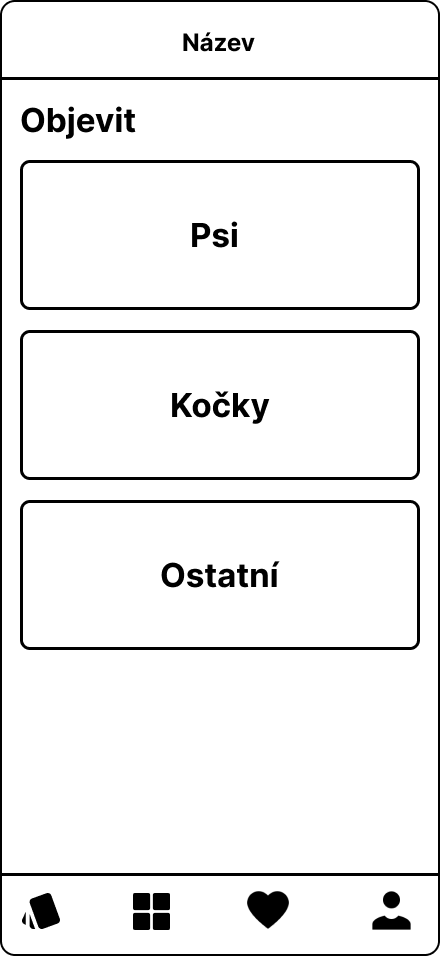
\includegraphics[width=0.25\textwidth]{img/explore.png}
    \caption{Návrh vyhledávací obrazovky aplikace.}
    \label{fig:explore_screen}
\end{figure}

Vyhledávací obrazovka je navržena s důrazem na intuitivní ovládání, přehlednost a rychlou navigaci mezi kategoriemi a detaily zvířat. Kombinace filtrů a skrolování umožňuje uživatelům efektivně najít požadované zvíře a pokračovat v adopčním procesu.

\subsection{Obrazovka oblíbených}

Obrazovka oblíbených poskytuje uživatelům přehled všech zvířat, která si označili jako oblíbená. Tato funkce usnadňuje opětovný přístup k vybraným zvířatům a jejich detailní prohlížení. 

Uživatel má možnost aplikovat jednoduchý filtr pro zobrazení specifických kategorií zvířat jako jsou psi, kočky nebo všechna zvířata.

Po výběru konkrétního zvířete se uživatel přesune na stránku s jeho detaily, kde může provádět další akce, jako je kontaktování útulku.

\begin{figure}[h!]
    \centering
    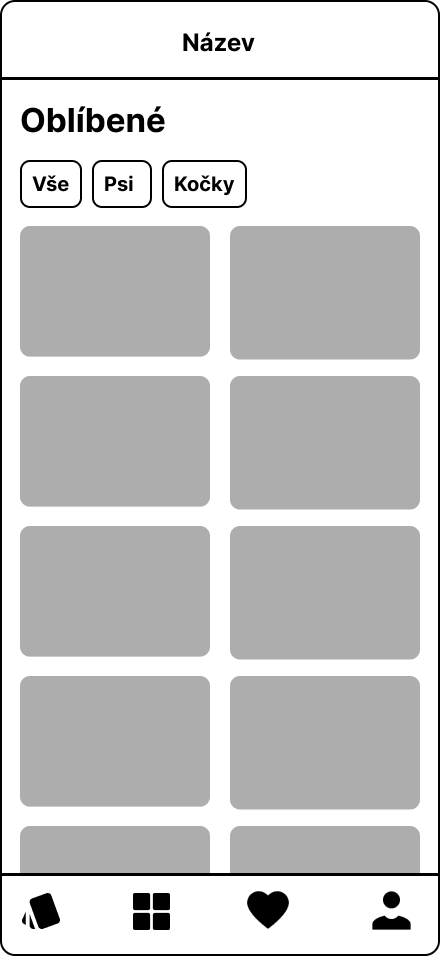
\includegraphics[width=0.25\textwidth]{img/like.png}
    \caption{Návrh vyhledávací obrazovky aplikace.}
    \label{fig:match_screen}
\end{figure}

\newpage

\subsection{Obrazovka profilu}

Obrazovka profilu slouží uživateli jako centrální místo pro správu jeho osobních údajů a nastavení aplikace. Uživatel zde může provádět následující akce:\\

\noindent \textbf{Úprava osobních informací}: Uživatel má možnost změnit své základní údaje, jako je jméno, e-mail nebo profilová fotografie.\\

\noindent \textbf{Přístup k nastavení}: Tlačítko pro přechod na stránku nastavení, kde lze přizpůsobit funkce aplikace (např. notifikace, jazyk rozhraní).\\

\noindent \textbf{Podpora a informace o aplikaci}: Možnost přesměrování na sekci technické podpory nebo zobrazení informací o aplikaci, včetně verzí a kontaktů na vývojářský tým.\\

\begin{figure}[h!]
    \centering
    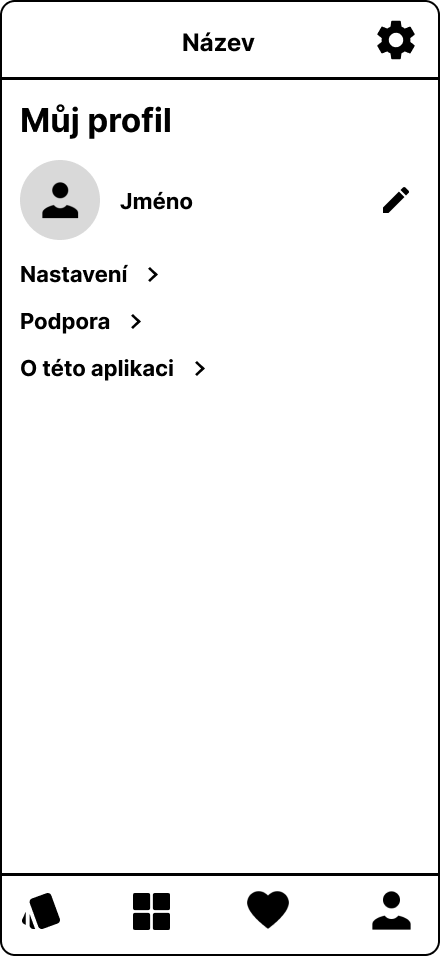
\includegraphics[width=0.25\textwidth]{img/account.png}
    \caption{Návrh obrazovky profilu v aplikaci.}
    \label{fig:profile_screen}
\end{figure}

Obrazovka profilu je navržena tak, aby uživatelům poskytla jednoduchý a přehledný přístup k osobním nastavením a informacím o aplikaci.

\newpage

\section{Výběr technologií a zdůvodnění volby}

\subsection{Použitá technologie pro vývoj aplikace}

Pro vývoj mobilní aplikace byla použita technologie React Native s frameworkem Expo. React Native umožňuje tvorbu multiplatformních aplikací pro Android i iOS s využitím jednoho kódu, přičemž výsledná aplikace dosahuje nativního výkonu díky využití nativních komponent. Technologie React Native je založena na knihovně React, což usnadňuje tvorbu modulárních a responzivních uživatelských rozhraní.

Framework Expo rozšiřuje funkcionalitu React Native o širokou škálu nástrojů a modulů, jako jsou navigace, přístup k senzorům a GPS nebo snadná integrace nativních funkcí. Expo rovněž umožňuje rychlý start projektu a jednoduché testování aplikace, čímž významně zefektivňuje celý proces vývoje. Tato kombinace poskytuje moderní, flexibilní a škálovatelné řešení pro vývoj mobilní aplikace.


\subsection{Použitá technologie pro backend}

Pro backend aplikace byla zvolena technologie Supabase, která poskytuje plně spravovanou PostgreSQL databázi s integrovanými funkcemi pro autentizaci, ukládání dat a synchronizaci v reálném čase. Supabase umožňuje snadné připojení k databázi a poskytuje nástroje pro správu uživatelských přístupů, uložení velkých souborů a zpracování požadavků v reálném čase.

Supabase dále nabízí bezpečnostní funkce, jako jsou Row Level Security politiky, které zajišťují granularitu přístupových práv k datům. Pro vývojáře je k dispozici sada klientských knihoven, které podporují různé programovací jazyky a platformy, což umožňuje snadnou integraci do aplikace. Tato technologie byla vybrána pro svou škálovatelnost, jednoduchou implementaci a robustní podporu vývoje moderních aplikací.


\section{Shrnutí návrhu}

Tato kapitola představila návrh mobilní aplikace zaměřené na inzerci a adopci domácích zvířat, která reaguje na identifikované nedostatky v současných softwarových řešeních. Hlavním cílem návrhu je vytvoření moderní, funkčně bohaté a uživatelsky přívětivé aplikace.

Nová aplikace je navržena s ohledem na klíčové funkční požadavky, jako jsou pokročilé filtrování zvířat, personalizovaná doporučení, optimalizace pro mobilní zařízení, snadná registrace uživatelů i útulků a správa dat v reálném čase. V rámci návrhu byly definovány uživatelské persony, které reprezentují hlavní cílové skupiny aplikace – zájemce o adopci a zaměstnance útulků. Tyto persony byly doplněny scénáři použití, které ilustrují nejčastější interakce uživatelů s aplikací.

Aplikace obsahuje několik klíčových obrazovek, mezi které patří hlavní obrazovka, vyhledávací obrazovka, sekce oblíbených a profilová obrazovka. Každá obrazovka byla detailně popsána a návrh byl podpořen ukázkami uživatelského rozhraní.

Pro vývoj aplikace byla zvolena technologie React Native společně s frameworkem Expo. Tato kombinace umožňuje efektivní vývoj multiplatformních aplikací pro Android a iOS s nativním výkonem a flexibilním uživatelským rozhraním. Backend aplikace je postaven na technologii Supabase, která poskytuje robustní řešení pro správu databáze, autentizaci, úložiště a synchronizaci dat v reálném čase. Tyto technologie byly vybrány pro jejich škálovatelnost, jednoduchou implementaci a podporu moderních vývojářských procesů.

Návrh aplikace a výběr použitých technologií tvoří základ pro realizaci komplexního a uživatelsky přívětivého řešení, které bude přínosné jak pro zájemce o adopci, tak pro útulky nabízející zvířata k adopci.


\chapter{Implementace}
\section{Přehled vývojového prostředí a nástrojů}
\section{Popis klíčových modulů a komponent}
\section{Implementace hlavních funkcí}
\section{Výzvy při vývoji a jejich řešení}

\chapter{Testování a ověření}
\section{Testovací metodologie}
\section{Testovací scénáře a případy}
\section{Shrnutí výsledků testování}

\chapter{Návrhy na budoucí rozšíření}
\section{Doporučené budoucí funkce nebo vylepšení}
\section{Možné integrace}
\section{Nápady na škálování aplikace}

\chapter{Závěr}
\section{Shrnutí provedené práce}
\section{Vyhodnocení aplikace vzhledem k původním cílům}
\section{Závěrečné zhodnocení a možnosti dalšího vývoje}

\appendix
\chapter{První příloha}

\printbibliography

\end{document}
